\subsection{Taxonomy-topic model}\label{sec:taxonomy_analysis}
Finally, we also want to analyze the taxonomy-topic model, especially since this model has the highest topic coherence out of all the tested models.
\autoref{tab:pachinko_selected_topics} shows selected lowest level topics from the the taxonomy-topic model.
As can be seen from the figure most of the topics are quite understandable.
However, there are some topics (e.g., topics 19 and 42) that consist entirely of words that provide little context or semantic meaning.
This indicates that the model has learned to group words that do not belong to any good topics.
This is a good feature that allows the model to apply an extra layer of preprocessing, automatically filtering away irrelevant words into topics.
This feature is also seen in some other topic models, such as in the hierarchical \gls{lda} (hLDA) by \citet{hLDA2004} and the embedded topic model (ETM) by \citet{dieng2020topic}, but the \gls{lda} does not seem to have this feature.

Since this model deals with more topic distributions than the other models, it is worth checking whether it also converges within the first 50 epochs, as with \gls{lda}.
This does seem to be the case, as indicated by \autoref{fig:pachinko_train}.
Here it can be seen that the topic coherence curve has flattened significantly, and thus additional epochs would yield diminishing returns.\vejleder{what about LL?}

\begin{figure}
	\centering
	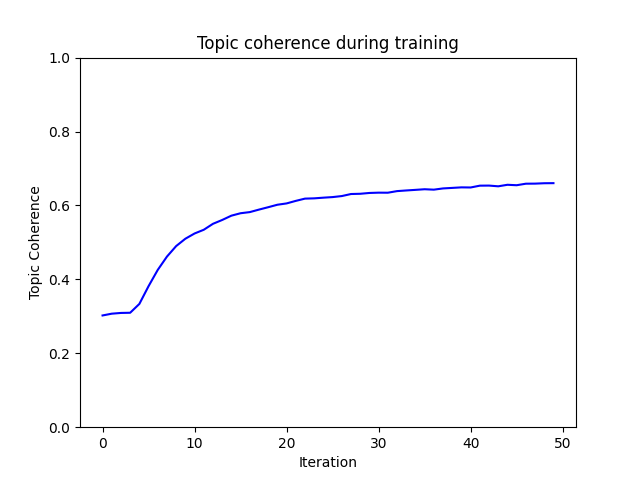
\includegraphics[width= \linewidth]{figures/pachinko_training.PNG}
	\caption{Topic coherence during training of the taxonomy-topic model.}
	\label{fig:pachinko_train}
\end{figure}

\autoref{tab:pachinko_mid_topics} gives an overview of how the taxonomy topics in the third layer of the taxonomy-topic model, are connected to the fourth layer topics that were generated by the model.
Some of these connections make a lot of sense, such as the 'Økonomi' (Economy) taxonomy entry topic which has the three filler topics (i.e., topics which consists entirely of words with little semantic value) within the top 5 most probable topics: 79, 75, and 42, as well as two topics which are about money: 74 and 9.
\autoref{tab:pachinko_selected_topics} shows the top words for each of these topics.
However not all the connections between higher and lower level topics are as understandable as these. 
For example, the 'Kriminalitet' (Crime) taxonomy entry has two filler topics within the 5 most probable topics: 42 and 75, one topic about economy: 60, one topic about politics: 8, and one topic about sports: 86.
\autoref{tab:pachinko_selected_topics} shows the top words for the topics mentioned in this section, and Appendix \autoref{tab:pachinko_topics} shows top words for all topics in the taxnomy-topic model.

Having the layered structure of the \gls{pam} gives many possibilities for recommending new articles to readers.
There is the possibility of exploring the similarity of taxonomies at the same layer and using this to recommend new articles with similar subjects.
For example, if an article is about 'Miljø' (environment) similar taxonomies might be 'Natur' (nature) and possibly 'Etik' (ethics), 'Trafik' (traffic), and 'Energi' (energy).

\begin{table*}[h]
	\centering
	\caption{Top 10 words of selected topics from our taxonomy-topic model. Labels have been manually added to the topics to increase readability.}
	\label{tab:pachinko_selected_topics}
	\begin{tabular}{c | c | c}
		Topic & Label & Top 10 words \\
		\hline
		8 & politics & venstre, valg, valget, partiet, partier, parti, stemmer, mette, politik, regering \\
		9 & money & procent, viser, tal, antallet, milliarder, pct, seneste, penge, millioner, indland \\
		19 & filler & mig, maske, du, folk, synes, ting, faktisk, nogen, altid, tror \\
		21 & university & unge, uddannelse, studerende, gymnasium, elever, uddannelser, universitet, procent, uddannelsen, nordjylland \\
		41 & academic research & universitet, professor, forskere, forskning, forskerne, viser, verden, institut, procent, aarhus \\
		42 & filler & mig, min, mit, ham, aldrig, gik, lille, maske, mine, altid \\
		45 & wildlife & dyr, naturen, natur, ulve, fugle, ulven, arter, dyrene, vilde, ulv \\
		47 & church & kirke, kirken, sognepræst, præst, søndag, koret, gudstjeneste, aften, kor, organist \\
		59 & music concerts & musik, koncert, sange, spiller, koncerter, band, koncerten, festival, musikken, publikum \\
		60 & buisness & virksomheden, millioner, a, direktør, procent, medarbejdere, selskabet, overskud, ansatte, virksomhed \\
		69 & primary school & elever, unge, skole, eleverne, skolen, skoler, klasse, børn, folkeskolen, lærere \\
		74 & elder care & ældre, borgere, kommunen, millioner, penge, nordjylland, plejehjem, borgerne, kommunens, budget \\
		75 & filler & du, din, dig, dit, altsa, dine, maske, nemlig, bruge, hvordan \\
		79 & filler & mig, min, hendes, hende, rigtig, arige, altid, arbejde, mor, mine \\
		86 & sports & handbold, mors, thy, hold, kamp, sæson, kampe, kampen, point, holdet \\
	\end{tabular}
\end{table*}


\begin{table*}[h]
	\centering
	\caption{IDs of the 5 most occurring fourth layer topics for each third layer topic from the pachinko model. See Appendix \autoref{tab:pachinko_topics} for the most occurring words for each ID.}
	\label{tab:pachinko_mid_topics}
	\begin{tabular}{c | c | c | c | c | c}
		Taxonomy Name & Top 5 Topic IDs & Taxonomy Name & Top 5 Topic IDs & Taxonomy Name & Top 5 Topic IDs \\ \hline
		Danmark & 8, 42, 82, 59, 79 & Udland & 42, 79, 59, 8, 32 & Kultur & 9, 42, 79, 19, 8 \\
		Landbrug & 42, 79, 8, 9, 19 & Kriminalitet & 42, 75, 60, 8, 86 & Socialstof & 42, 9, 79, 86, 8 \\
		Arbejdsmarked & 42, 79, 59, 8, 9 & Økonomi & 79, 75, 74, 42, 9 & Sundhed & 8, 32, 42, 9, 19 \\
		Politik & 42, 75, 9, 19, 74 & Musik & 75, 42, 59, 11, 79 & Sport & 42, 75, 8, 59, 52 \\
		Bolig & 75, 42, 86, 79, 8 & Videnskab & 42, 8, 52, 79, 19 & Trafik & 42, 74, 8, 52, 32 \\
		Erhverv & 42, 8, 59, 32, 79 & Uddannelse & 42, 9, 75, 32, 74 & Energi & 42, 8, 79, 19, 86 \\
		Ulykker & 42, 75, 9, 79, 32 & Fritid & 42, 8, 75, 82, 79 & Socialt & 42, 75, 79, 59, 9 \\
		Dyr & 86, 42, 79, 52, 9 & Natur & 42, 52, 9, 32, 79 & Miljø & 8, 42, 75, 52, 59 \\
		Familie & 79, 8, 42, 59, 32 & Politi & 42, 75, 79, 8, 59 & Byggeri & 75, 42, 79, 77, 59 \\
		Etik & 79, 42, 8, 86, 74 & Religion & 42, 79, 8, 59, 32 & Kommunalvalg & 42, 8, 75, 79, 32 \\
		Nordjyske Plus & 42, 86, 9, 79, 74 & DF & 42, 8, 59, 52, 19 & & \\
	\end{tabular}
\end{table*}
